\chapter{Bio.PopGen: Population genetics}

Bio.PopGen is a Biopython module supporting population genetics,
available in Biopython 1.44 onwards.

The medium term objective for the module is to support widely used data
formats, applications and databases. This module is currently under intense
development and support for new features should appear at a rather fast pace.
Unfortunately this might also entail some instability on the API, especially
if you are using a development version. APIs that are made available on
our official public releases should be much more stable.

\section{GenePop}

GenePop (\url{http://genepop.curtin.edu.au/}) is a popular population
genetics software package supporting Hardy-Weinberg tests, linkage
desiquilibrium, population diferentiation, basic statistics, $F_{st}$ and
migration estimates, among others. GenePop does not supply sequence
based statistics as it doesn't handle sequence data.
The GenePop file format is supported by a wide range of other population
genetic software applications, thus making it a relevant format in the
population genetics field.

Bio.PopGen provides a parser and generator of GenePop file format.
Utilities to manipulate the content of a record are also provided.
Here is an example on how to read a GenePop file (you can find
example GenePop data files in the Test/PopGen directory of Biopython):

\begin{verbatim}
from Bio.PopGen import GenePop

handle = open("example.gen")
rec = GenePop.read(handle)
handle.close()
\end{verbatim}

This will read a file called example.gen and parse it. If you
do print rec, the record will be output again, in GenePop format.

The most important information in rec will be the loci names and
population information (but there is more -- use help(GenePop.Record)
to check the API documentation). Loci names can be found on rec.loci\_list.
Population information can be found on rec.populations.
Populations is a list with one element per population. Each element is itself
a list of individuals, each individual is a pair composed by individual
name and a list of alleles (2 per marker), here is an example for
rec.populations:

\begin{verbatim}
[
    [
        ('Ind1', [(1, 2),    (3, 3), (200, 201)],
        ('Ind2', [(2, None), (3, 3), (None, None)],
    ],
    [
        ('Other1', [(1, 1),  (4, 3), (200, 200)],
    ]
]
\end{verbatim}

So we have two populations, the first with two individuals, the
second with only one. The first individual of the first
population is called Ind1, allelic information for each of
the 3 loci follows. Please note that for any locus, information
might be missing (see as an example, Ind2 above).

A few utility functions to manipulate GenePop records are made
available, here is an example:

\begin{verbatim}
from Bio.PopGen import GenePop

#Imagine that you have loaded rec, as per the code snippet above...

rec.remove_population(pos)
#Removes a population from a record, pos is the population position in
#  rec.populations, remember that it starts on position 0.
#  rec is altered.

rec.remove_locus_by_position(pos)
#Removes a locus by its position, pos is the locus position in
#  rec.loci_list, remember that it starts on position 0.
#  rec is altered.

rec.remove_locus_by_name(name)
#Removes a locus by its name, name is the locus name as in
#  rec.loci_list. If the name doesn't exist the function fails
#  silently.
#  rec is altered.

rec_loci = rec.split_in_loci()
#Splits a record in loci, that is, for each loci, it creates a new
#  record, with a single loci and all populations.
#  The result is returned in a dictionary, being each key the locus name.
#  The value is the GenePop record.
#  rec is not altered.

rec_pops =  rec.split_in_pops(pop_names)
#Splits a record in populations, that is, for each population, it creates
#  a new record, with a single population and all loci.
#  The result is returned in a dictionary, being each key
#  the population name. As population names are not available in GenePop,
#  they are passed in array (pop_names).
#  The value of each dictionary entry is the GenePop record.
#  rec is not altered.
\end{verbatim}

GenePop does not support population names, a limitation which can be
cumbersome at times. Functionality to enable population names is currently
being planned for Biopython. These extensions won't break compatibility in
any way with the standard format.  In the medium term, we would also like to
support the GenePop web service.

\section{Coalescent simulation}

A coalescent simulation is a backward model of population genetics with relation to
time. A simulation of ancestry is done until the Most Recent Common Ancestor (MRCA) is found.
This ancestry relationship starting on the MRCA and ending on the current generation
sample is sometimes called a genealogy. Simple cases assume a population of constant
size in time, haploidy, no population structure, and simulate the alleles of a single
locus under no selection pressure.

Coalescent theory is used in many fields like selection detection, estimation of
demographic parameters of real populations or disease gene mapping.

The strategy followed in the Biopython implementation of the coalescent was not
to create a new, built-in, simulator from scratch but to use an existing one,
Fastsimcoal2 (\url{http://cmpg.unibe.ch/software/fastsimcoal2/}). Fastsimcoal2 allows for,
among others, population structure, multiple demographic events, simulation
of multiple types of loci (SNPs, sequences, STRs/microsatellites and RFLPs)
with recombination, diploidy multiple chromosomes or ascertainment bias. Notably
Fastsimcoal2 doesn't support any selection model. We recommend reading
Fastsimcoal2's
documentation, available in the link above.

The input for Fastsimcoal2 is a file specifying the desired demography and genome,
the output is a set of files (typically around 1000) with the simulated genomes
of a sample of individuals per subpopulation. This set of files can be used
in many ways, like to compute confidence intervals where which certain
statistics (e.g., $F_{st}$ or Tajima D) are expected to lie. Real population
genetics datasets statistics can then be compared to those confidence intervals.

Biopython coalescent code allows to create demographic scenarios and genomes and
to run Fastsimcoal2.

\subsection{Creating scenarios}

Creating a scenario involves both creating a demography and a chromosome structure.
In many cases (e.g. when doing Approximate Bayesian Computations -- ABC) it is
important to test many parameter variations (e.g. vary the effective population size,
$N_e$, between 10, 50, 500 and 1000 individuals). The code provided allows for
the simulation of scenarios with different demographic parameters very easily.

Below we see how we can create scenarios and then how simulate them.

\subsubsection{Demography}

A few predefined demographies are built-in, all have two shared parameters: sample size
(called sample\_size on the template, see below for its use) per deme and deme size, i.e.
subpopulation size (pop\_size). All demographies are available as templates where all
parameters can be varied, each template has a system name. The prefedined
demographies/templates are:

\begin{description}
\item[Single population, constant size] The standard parameters are enough to specify
it. Template name: simple.
\item[Single population, bottleneck] As seen on figure \ref{fig:bottle}. The parameters
are current population size (pop\_size on template ne3 on figure), time of expansion,
given as the generation in the past when it occurred (expand\_gen),
effective population size during bottleneck (ne2), time of contraction
(contract\_gen) and original size in the remote past (ne3). Template name: bottle.
\item[Island model] The typical island model. The total number of demes is specified
by total\_demes and the migration rate by mig. Template name island.
\item[Stepping stone model - 1 dimension] The stepping stone model in 1 dimension,
extremes disconnected. The total number of demes is total\_demes, migration rate
is mig. Template name is ssm\_1d.
\item[Stepping stone model - 2 dimensions] The stepping stone model in 2 dimensions,
extremes disconnected. The parameters are x for the horizontal dimension and y
for the vertical (being the total number of demes x times y), migration rate is mig.
Template name is ssm\_2d.
\end{description}

\begin{htmlonly}
\label{fig:bottle}
\imgsrc{images/bottle.png}
\end{htmlonly}

\begin{latexonly}
\begin{figure}[htbp]
\centering
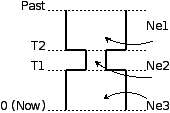
\includegraphics{images/bottle.png}
\caption{A bottleneck}
\label{fig:bottle}
\end{figure}
\end{latexonly}

In our first example, we will generate a template for a single population, constant size
model with a sample size of 30 and a deme size of 500. The code for this is:

\begin{verbatim}
from Bio.PopGen.SimCoal.Template import generate_simcoal_from_template

generate_simcoal_from_template('simple',
    [(1, [('SNP', [24, 0.0005, 0.0])])],
    [('sample_size', [30]),
    ('pop_size', [100])])
\end{verbatim}

Executing this code snippet will generate a file on the current directory called
simple\_100\_300.par this file can be given as input to Fastsimcoal2 to simulate the
demography (below we will see how Biopython can take care of calling
Fastsimcoal2).

This code consists of a single function call, let's discuss it parameter by parameter.

The first parameter is the template id (from the list above). We are using the id
'simple' which is the template for a single population of constant size along time.

The second parameter is the chromosome structure. Please ignore it for now, it will be
explained in the next section.

The third parameter is a list of all required parameters (recall that the simple model
only needs sample\_size and pop\_size) and possible values (in this case each
parameter only has a possible value).

Now, let's consider an example where we want to generate several island models, and we
are interested in varying the number of demes: 10, 50 and 100 with a migration
rate of 1\%. Sample size and deme
size will be the same as before. Here is the code:


\begin{verbatim}
from Bio.PopGen.SimCoal.Template import generate_simcoal_from_template

generate_simcoal_from_template('island',
    [(1, [('SNP', [24, 0.0005, 0.0])])],
    [('sample_size', [30]),
    ('pop_size', [100]),
    ('mig', [0.01]),
    ('total_demes', [10, 50, 100])])
\end{verbatim}

In this case, 3 files will be generated: island\_100\_0.01\_100\_30.par,
island\_10\_0.01\_100\_30.par and island\_50\_0.01\_100\_30.par. Notice the
rule to make file names: template name, followed by parameter values in
reverse order.

A few, arguably more esoteric template demographies exist (please check the
Bio/PopGen/SimCoal/data directory on Biopython source tree). Furthermore it is possible
for the user to create new templates. That functionality will be discussed in a future
version of this document.

\subsubsection{Chromosome structure}

We strongly recommend reading Fastsimcoal2 documentation to understand the full potential
available in modeling chromosome structures. In this subsection we only discuss how
to implement chromosome structures using the Biopython interface, not the underlying
Fastsimcoal2 capabilities.

We will start by implementing a single chromosome, with 24 SNPs with
a recombination rate immediately on the right of each locus of 0.0005 and a
minimum frequency of the minor allele of 0. This will be specified by the
following list (to be passed as second parameter to the function
generate\_simcoal\_from\_template):

\begin{verbatim}
[(1, [('SNP', [24, 0.0005, 0.0])])]
\end{verbatim}

This is actually the chromosome structure used in the above examples.


The chromosome structure is represented by a list of chromosomes,
each chromosome (i.e., each element in the list)
is composed by a tuple (a pair): the first element
is the number of times the chromosome is to be repeated (as there
might be interest in repeating the same chromosome many times).
The second element is a list of the actual components of the chromosome.
Each element is again a pair, the first member is the locus type and
the second element the parameters for that locus type. Confused?
Before showing more examples let's review the example above: We have
a list with one element (thus one chromosome), the chromosome is
a single instance (therefore not to be repeated), it is composed
of 24 SNPs, with a recombination rate of 0.0005 between each
consecutive SNP, the minimum frequency of the minor allele is
0.0 (i.e, it can be absent from a certain population).

Let's see a more complicated example:

\begin{verbatim}
[
  (5, [
       ('SNP', [24, 0.0005, 0.0])
      ]
  ),
  (2, [
       ('DNA', [10, 0.0, 0.00005, 0.33]),
       ('RFLP', [1, 0.0, 0.0001]),
       ('MICROSAT', [1, 0.0, 0.001, 0.0, 0.0])
      ]
  )
]
\end{verbatim}

We start by having 5 chromosomes with the same structure as
above (i.e., 24 SNPs). We then have 2 chromosomes which
have a DNA sequence with 10 nucleotides, 0.0 recombination rate,
0.0005 mutation rate, and a transition rate of 0.33. Then we
have an RFLP with 0.0 recombination rate to the next locus and
a 0.0001 mutation rate. Finally we have a microsatellite (or STR),
with 0.0 recombination rate to the next locus (note, that as this
is a single microsatellite which has no loci following, this
recombination rate here is irrelevant), with a mutation rate
of 0.001, geometric parameter of 0.0 and a range constraint
of 0.0 (for information about this parameters please consult
the Fastsimcoal2 documentation, you can use them to simulate
various mutation models, including the typical  -- for microsatellites --
stepwise mutation model among others).


\subsection{Running Fastsimcoal2}

We now discuss how to run Fastsimcoal2 from inside Biopython. It is required
that the binary for Fastsimcoal2 is called fastsimcoal21 (or fastsimcoal21.exe on Windows
based platforms), please note that the typical name when downloading the
program is in the format fastsimcoal2\_x\_y. As such, when installing
Fastsimcoal2
you will need to rename of the downloaded executable so that Biopython can
find it.

It is possible to run Fastsimcoal2 on files that were not generated using the method
above (e.g., writing a parameter file by hand), but we will show an
example by creating a model using the framework presented above.

\begin{verbatim}
from Bio.PopGen.SimCoal.Template import generate_simcoal_from_template
from Bio.PopGen.SimCoal.Controller import FastSimCoalController


generate_simcoal_from_template('simple',
    [
      (5, [
           ('SNP', [24, 0.0005, 0.0])
          ]
      ),
      (2, [
           ('DNA', [10, 0.0, 0.00005, 0.33]),
           ('RFLP', [1, 0.0, 0.0001]),
           ('MICROSAT', [1, 0.0, 0.001, 0.0, 0.0])
          ]
      )
    ],
    [('sample_size', [30]),
    ('pop_size', [100])])

ctrl = FastSimCoalController()
ctrl.run_fastsimcoal('simple_100_30.par', 50)
\end{verbatim}

The lines of interest are the last two (plus the new import).
Firstly a controller for the
application is created. The directory where the binary is located has
to be specified.

The simulator is then run on the last line: we know, from the rules explained
above, that the input file name is simple\_100\_30.par for the
simulation parameter file created. We then specify
that we want to run 50 independent simulations, by default Biopython
requests a simulation of diploid data, but a third parameter can
be added to simulate haploid data (adding as a parameter the
string '0'). Fastsimcoal2 will now run (please
note that this can take quite a lot of time) and will create a directory
with the simulation results. The results can now be analysed (typically
studying the data with Arlequin3). In the future Biopython might support
reading the Arlequin3 format and thus allowing for the analysis of
Fastsimcoal2
data inside Biopython.


\section{Other applications}

Here we discuss interfaces and utilities to deal with population genetics'
applications which arguably have a smaller user base.

\subsection{FDist: Detecting selection and molecular adaptation}

FDist is a selection detection application suite based on computing
(i.e. simulating) a ``neutral'' confidence interval based on $F_{st}$ and
heterozygosity. Markers (which can be SNPs, microsatellites, AFLPs
among others) which lie outside the ``neutral'' interval are to be
considered as possible candidates for being under selection.

FDist is mainly used when the number of markers is considered enough
to estimate an average $F_{st}$, but not enough to either have outliers
calculated from the dataset directly or, with even more markers for
which the relative positions in the genome are known, to use
approaches based on, e.g., Extended Haplotype Heterozygosity (EHH).

The typical usage pattern for FDist is as follows:

\begin{enumerate}
\item Import a dataset from an external format into FDist format.
\item Compute average $F_{st}$. This is done by datacal inside FDist.
\item Simulate ``neutral'' markers based on the
    average $F_{st}$ and expected number of total populations.
    This is the core operation, done by fdist inside FDist.
\item Calculate the confidence interval, based on the desired
    confidence boundaries (typically 95\% or 99\%). This is done by
    cplot and is mainly used to plot the interval.
\item Assess each marker status against the simulation ``neutral''
    confidence interval. Done
    by pv. This is used to detect the outlier status of each marker
    against the simulation.
\end{enumerate}

We will now discuss each step with illustrating example code
(for this example to work FDist binaries have to be on the
executable PATH).

The FDist data format is application specific and is not used at
all by other applications, as such you will probably have to convert
your data for use with FDist. Biopython can help you do this.
Here is an example converting from GenePop format to FDist format
(along with imports that will be needed on examples further below):

\begin{verbatim}
from Bio.PopGen import GenePop
from Bio.PopGen import FDist
from Bio.PopGen.FDist import Controller
from Bio.PopGen.FDist.Utils import convert_genepop_to_fdist

gp_rec = GenePop.read(open("example.gen"))
fd_rec = convert_genepop_to_fdist(gp_rec)
in_file = open("infile", "w")
in_file.write(str(fd_rec))
in_file.close()
\end{verbatim}

In this code we simply parse a GenePop file and convert it to a FDist
record.

Printing an FDist record will generate
a string that can be directly saved to a file and supplied to FDist. FDist
requires the input file to be called infile, therefore we save the record on
a file with that name.

The most important fields on a FDist record are: num\_pops, the number of
populations; num\_loci, the number of loci and loci\_data with the marker
data itself. Most probably the details of the record are of no interest
to the user, as the record only purpose is to be passed to FDist.

The next step is to calculate the average $F_{st}$ of the dataset (along
with the sample size):

\begin{verbatim}
ctrl = Controller.FDistController()
fst, samp_size = ctrl.run_datacal()
\end{verbatim}

On the first line we create an object to control the call of  FDist
suite, this object will be used further on in order to call other
suite applications.

On the second line we call the datacal application which computes the
average $F_{st}$
and the sample size. It is worth noting that the $F_{st}$ computed by
datacal is a \emph{variation} of Weir and Cockerham's $\theta$.

We can now call the main fdist application in order to simulate neutral
markers.

\begin{verbatim}
sim_fst = ctrl.run_fdist(npops = 15, nsamples = fd_rec.num_pops, fst = fst,
    sample_size = samp_size, mut = 0, num_sims = 40000)
\end{verbatim}

\begin{description}
\item[npops] Number of populations existing in nature. This is really a
    ``guestimate''. Has to be lower than 100.
\item[nsamples] Number of populations sampled, has to be lower than npops.
\item[fst] Average $F_{st}$.
\item[sample\_size] Average number of individuals sampled on each population.
\item[mut] Mutation model: 0 - Infinite alleles; 1 - Stepwise mutations
\item[num\_sims] Number of simulations to perform. Typically a number around
    40000 will be OK, but if you get a confidence interval that looks sharp
    (this can be detected when plotting the confidence interval computed
    below) the value can be increased (a suggestion would be steps of 10000
    simulations).
\end{description}

The confusion in wording between number of samples and sample size
stems from the original application.

A file named out.dat will be created with the simulated heterozygosities
and $F_{st}$s, it will have as many lines as the number of simulations
requested.

Note that fdist returns the average $F_{st}$ that it was \emph{capable} of
simulating, for more details about this issue please read below the paragraph
on approximating the desired average $F_{st}$.

The next (optional) step is to calculate the confidence interval:

\begin{verbatim}
cpl_interval = ctrl.run_cplot(ci=0.99)
\end{verbatim}

You can only call cplot after having run fdist.

This will calculate the confidence intervals (99\% in this case)
for a previous fdist run. A list of quadruples is returned. The
first element represents the heterozygosity, the second the lower
bound of $F_{st}$ confidence interval for that heterozygosity,
the third the average and the fourth the upper bound. This can
be used to trace the confidence interval contour. This list
is also written to a file, out.cpl.

The main purpose of this step is return a set of points which can
be easily used to plot a confidence interval. It can be skipped
if the objective is only to assess the status of each marker against
the simulation, which is the next step...

\begin{verbatim}
pv_data = ctrl.run_pv()
\end{verbatim}

You can only call cplot after having run datacal and fdist.

This will use the simulated markers to assess the status of each
individual real marker. A list, in the same order than the loci\_list
that is on the FDist record (which is in the same order that the GenePop
record) is returned. Each element in the list is a quadruple, the
fundamental member of each quadruple is the last element (regarding the
other elements, please refer to the pv documentation -- for the
sake of simplicity we will not discuss them here) which returns the
probability of the simulated $F_{st}$ being lower than the marker $F_{st}$.
Higher values would indicate a stronger candidate for positive selection,
lower values a candidate for balancing selection, and intermediate values
a possible neutral marker. What is ``higher'', ``lower'' or ``intermediate''
is really a subjective issue, but taking a ``confidence interval'' approach
and considering a 95\% confidence interval, ``higher'' would be between 0.95
and 1.0, ``lower'' between 0.0 and 0.05 and ``intermediate'' between 0.05 and
0.95.

\subsubsection{Approximating the desired average $F_{st}$}

Fdist tries to approximate the desired average $F_{st}$ by doing a
coalescent simulation using migration rates based on the formula

\[ N_{m} = \frac{1 - F_{st}}{4F_{st}} \]

This formula assumes a few premises like an infinite number of populations.

In practice, when the number of populations is low, the mutation model
is stepwise and the sample size increases, fdist will not be able to
simulate an acceptable approximate average $F_{st}$.

To address that, a function is provided to iteratively approach the desired
value by running several fdists in sequence. This approach is computationally
more intensive than running a single fdist run, but yields good results.
The following code runs fdist approximating the desired $F_{st}$:

\begin{verbatim}
sim_fst = ctrl.run_fdist_force_fst(npops = 15, nsamples = fd_rec.num_pops,
    fst = fst, sample_size = samp_size, mut = 0, num_sims = 40000,
    limit = 0.05)
\end{verbatim}

The only new optional parameter, when comparing with run\_fdist, is limit
which is the desired maximum error. run\_fdist can (and probably should)
be safely replaced with run\_fdist\_force\_fst.

\subsubsection{Final notes}

The process to determine the average $F_{st}$ can be more sophisticated than
the one presented here. For more information we refer you to the FDist
README file. Biopython's code can be used to implement more sophisticated
approaches.

\section{Future Developments}

The most desired future developments would be the ones you add yourself ;) .

That being said, already existing fully functional code is currently being
incorporated in Bio.PopGen, that code covers the applications FDist and
SimCoal2, the HapMap and UCSC Table Browser databases and some simple statistics
like $F_{st}$, or allele counts.

